\documentclass[a4paper,10pt]{article}
\usepackage[utf8]{inputenc}
\usepackage[slovene]{babel}
\usepackage{graphicx}
\usepackage{hyperref}
\usepackage[left=2cm,right=2cm,top=2cm,bottom=3cm]{geometry}
\usepackage{amsmath}
\usepackage{float}
\usepackage{bbold}

\makeatletter
\renewcommand*\env@matrix[1][*\c@MaxMatrixCols c]{%
  \hskip -\arraycolsep
  \let\@ifnextchar\new@ifnextchar
  \array{#1}}
\makeatother

%opening
\title{Modelekularna dinamika}
\author{Miha \v Can\v cula}

\newcommand{\uvec}[1]{\ensuremath{\underline{#1}}}
\newcommand{\bb}{
  \ensuremath{b_1 b_2 \ldots b_n}
}
\newcommand{\psibb}{
  \ensuremath{\psi_{\bb}}
}

\begin{document}

\maketitle

\section{Transport toplote}

Transport toplote sem preu"ceval z enodimenzionalno verigo oscilatorjev. 
Delca na konceh verige sem sklopil s toplotnima kopelima z brezdimenzijskima temperaturama $T_L=1$ in $T_R=2$. 

Zanimajo nas vrednosti v stacionarnem stanju, zato sem najprej napravil $N_I = 10^{8}$ korakov integracije dol"zine $h=10^{-2}$. 
Nato sem izvedel "se $N_A=10^{7}$ korakov, med katerimi sem opravil $10^{5}$ meritev temperature in toplotnega toka. 
Meritve sem na koncu popre"cil. 

\section{Maxwellske kopeli}

Najprej sem za modeliranje toplotnih kopeli uporabil Maxwellov algoritem, pri katerem gibalni koli"cini sklopljenih delcev resetiramo vsakih $R=100$ korakov. 
Preizku"sal sem razli"cne vrednosti za $R$, najbolje pa se je izkazala tak"sna, pri kateri se reset zgodi enkrat vsako "casovno enoto, torej $Rh \sim 1$. 
Med reseti sem stanje propagiral s simplekti"cnim integratorjem s simetri"cno shemo $S_2$. 

\begin{figure}[H]
 \centering
 \input{g_odv_lambda_30}
  \caption{Temperaturni profil v odvisnosti od parametra $\lambda$ za sistem s 30 delci}
\end{figure}


"Ze pri srednji velikosti sistema ($N=30$) opazimo odvisnost temperaturne porazdelitve od motnje $\lambda$. 
Veriga povsem harmoni"cnih oscilatorjev ($\lambda=0$) ima povsod, razen na obeh konceh, povpre"cno temperaturo. 
Pri $\lambda$ nad 1 temperatura med obema koncema nara"s"ca linearno, brez skokov. 
Pri vmesnih vrednosti pa opazimo kombinacijo obeh pojavov: na konceh ima temperatura diskretne skoke, vmes pa nara"s"ca linearno. 

Zelo podoben pojav opazimo tudi z ve"cjim sistemom, na primer $N=100$ na spodnji sliki. 


\begin{figure}[H]
 \centering
 \input{g_odv_lambda_100}
  \caption{Temperaturni profil v odvisnosti od parametra $\lambda$ za sistem s 100 delci}
\end{figure}

Za oceno termodinamske limite je zanimiva tudi odvisnost od velikosti sistema. 
Pri konstantnem parametru $\lambda = 0.6$ pri ve"cjem sistemu opazimo vedno manj"se robne skoke. 

\begin{figure}[H]
 \centering
 \input{g_odv_velikost}
\caption{Temperaturni profil pri fiksnem $\lambda = 0.6$ in razli"cnih velikostih sistema}
\end{figure}


Na prej"snjih slikah smo videli, da je temperaturni profil odvisen predvsem od motnje $\lambda$. 
Opazujemo lahko prehod med stanjem s konstantno temperaturo transportom ($\lambda=1$) in stanjem z linearnim profilom ($\lambda=1$). 
Z ve"canjem velikosti sistema $N$ postanejo za"cetni skoki pri srednji $\lambda$ vedno manj izraziti, zato domnevam,
da v limiti $N\to\infty$ nastane oster prehod med konstantnim in linearnim profilom. 

Polo"zaj prehoda sem posku"sal najti tako, da sem opazoval temperaturo v to"cki na 1/5 verige v odvisnosti od $\lambda$ in $N$. 
Rezultati so na spodnji sliki. 

\begin{figure}[H]
 \centering
 % GNUPLOT: LaTeX picture with Postscript
\begingroup
  \makeatletter
  \providecommand\color[2][]{%
    \GenericError{(gnuplot) \space\space\space\@spaces}{%
      Package color not loaded in conjunction with
      terminal option `colourtext'%
    }{See the gnuplot documentation for explanation.%
    }{Either use 'blacktext' in gnuplot or load the package
      color.sty in LaTeX.}%
    \renewcommand\color[2][]{}%
  }%
  \providecommand\includegraphics[2][]{%
    \GenericError{(gnuplot) \space\space\space\@spaces}{%
      Package graphicx or graphics not loaded%
    }{See the gnuplot documentation for explanation.%
    }{The gnuplot epslatex terminal needs graphicx.sty or graphics.sty.}%
    \renewcommand\includegraphics[2][]{}%
  }%
  \providecommand\rotatebox[2]{#2}%
  \@ifundefined{ifGPcolor}{%
    \newif\ifGPcolor
    \GPcolortrue
  }{}%
  \@ifundefined{ifGPblacktext}{%
    \newif\ifGPblacktext
    \GPblacktexttrue
  }{}%
  % define a \g@addto@macro without @ in the name:
  \let\gplgaddtomacro\g@addto@macro
  % define empty templates for all commands taking text:
  \gdef\gplbacktext{}%
  \gdef\gplfronttext{}%
  \makeatother
  \ifGPblacktext
    % no textcolor at all
    \def\colorrgb#1{}%
    \def\colorgray#1{}%
  \else
    % gray or color?
    \ifGPcolor
      \def\colorrgb#1{\color[rgb]{#1}}%
      \def\colorgray#1{\color[gray]{#1}}%
      \expandafter\def\csname LTw\endcsname{\color{white}}%
      \expandafter\def\csname LTb\endcsname{\color{black}}%
      \expandafter\def\csname LTa\endcsname{\color{black}}%
      \expandafter\def\csname LT0\endcsname{\color[rgb]{1,0,0}}%
      \expandafter\def\csname LT1\endcsname{\color[rgb]{0,1,0}}%
      \expandafter\def\csname LT2\endcsname{\color[rgb]{0,0,1}}%
      \expandafter\def\csname LT3\endcsname{\color[rgb]{1,0,1}}%
      \expandafter\def\csname LT4\endcsname{\color[rgb]{0,1,1}}%
      \expandafter\def\csname LT5\endcsname{\color[rgb]{1,1,0}}%
      \expandafter\def\csname LT6\endcsname{\color[rgb]{0,0,0}}%
      \expandafter\def\csname LT7\endcsname{\color[rgb]{1,0.3,0}}%
      \expandafter\def\csname LT8\endcsname{\color[rgb]{0.5,0.5,0.5}}%
    \else
      % gray
      \def\colorrgb#1{\color{black}}%
      \def\colorgray#1{\color[gray]{#1}}%
      \expandafter\def\csname LTw\endcsname{\color{white}}%
      \expandafter\def\csname LTb\endcsname{\color{black}}%
      \expandafter\def\csname LTa\endcsname{\color{black}}%
      \expandafter\def\csname LT0\endcsname{\color{black}}%
      \expandafter\def\csname LT1\endcsname{\color{black}}%
      \expandafter\def\csname LT2\endcsname{\color{black}}%
      \expandafter\def\csname LT3\endcsname{\color{black}}%
      \expandafter\def\csname LT4\endcsname{\color{black}}%
      \expandafter\def\csname LT5\endcsname{\color{black}}%
      \expandafter\def\csname LT6\endcsname{\color{black}}%
      \expandafter\def\csname LT7\endcsname{\color{black}}%
      \expandafter\def\csname LT8\endcsname{\color{black}}%
    \fi
  \fi
  \setlength{\unitlength}{0.0500bp}%
  \begin{picture}(7200.00,5040.00)%
    \gplgaddtomacro\gplbacktext{%
      \csname LTb\endcsname%
      \put(1078,704){\makebox(0,0)[r]{\strut{} 1.3}}%
      \put(1078,1518){\makebox(0,0)[r]{\strut{} 1.35}}%
      \put(1078,2332){\makebox(0,0)[r]{\strut{} 1.4}}%
      \put(1078,3147){\makebox(0,0)[r]{\strut{} 1.45}}%
      \put(1078,3961){\makebox(0,0)[r]{\strut{} 1.5}}%
      \put(1078,4775){\makebox(0,0)[r]{\strut{} 1.55}}%
      \put(1210,484){\makebox(0,0){\strut{} 0}}%
      \put(1909,484){\makebox(0,0){\strut{} 0.02}}%
      \put(2608,484){\makebox(0,0){\strut{} 0.04}}%
      \put(3307,484){\makebox(0,0){\strut{} 0.06}}%
      \put(4007,484){\makebox(0,0){\strut{} 0.08}}%
      \put(4706,484){\makebox(0,0){\strut{} 0.1}}%
      \put(5405,484){\makebox(0,0){\strut{} 0.12}}%
      \put(6104,484){\makebox(0,0){\strut{} 0.14}}%
      \put(6803,484){\makebox(0,0){\strut{} 0.16}}%
      \put(176,2739){\rotatebox{-270}{\makebox(0,0){\strut{}$T(1/5)$}}}%
      \put(4006,154){\makebox(0,0){\strut{}$\lambda$}}%
    }%
    \gplgaddtomacro\gplfronttext{%
      \csname LTb\endcsname%
      \put(2266,1977){\makebox(0,0)[r]{\strut{}$N = 10$}}%
      \csname LTb\endcsname%
      \put(2266,1757){\makebox(0,0)[r]{\strut{}$N = 20$}}%
      \csname LTb\endcsname%
      \put(2266,1537){\makebox(0,0)[r]{\strut{}$N = 30$}}%
      \csname LTb\endcsname%
      \put(2266,1317){\makebox(0,0)[r]{\strut{}$N = 50$}}%
      \csname LTb\endcsname%
      \put(2266,1097){\makebox(0,0)[r]{\strut{}$N = 100$}}%
      \csname LTb\endcsname%
      \put(2266,877){\makebox(0,0)[r]{\strut{}$N = 200$}}%
    }%
    \gplbacktext
    \put(0,0){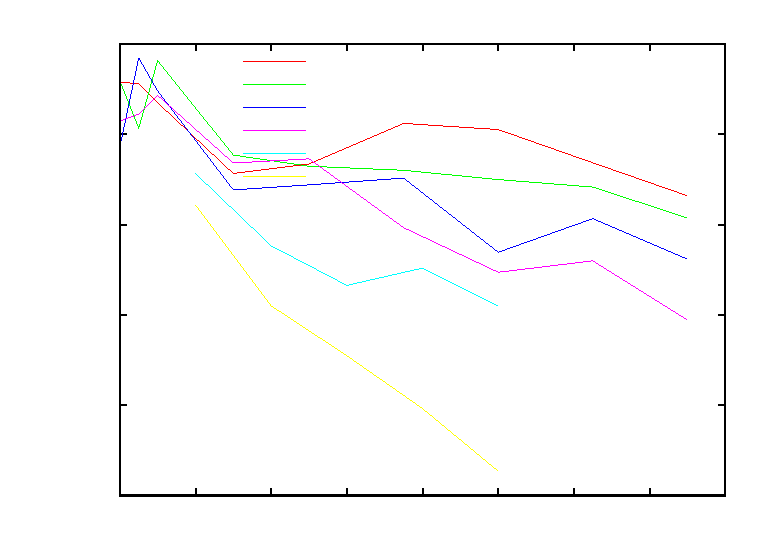
\includegraphics{g_prehod}}%
    \gplfronttext
  \end{picture}%
\endgroup

  \caption{Iskanje faznega prehoda med konstantnim in linearnim profilom}
\end{figure}

Dokler je $\lambda$ manj"sa od neke kriti"cne vrednosti, ki je nekje okrog $0.01$, temperatura ni odvisna niti od $\lambda$ niti od $N$. 
Nad to mejo pa temperatura pada z $\lambda$, in to hitreje pri ve"cjih $N$. 
To se sklada z domnevo, da v termodinamski limiti dobimo oster prehod. 
Na podlagi mojih izra"cunov mi ni uspelo dolo"citi natan"cnega polo"zaja prehoda, niti ne morem z gotovostjo trditi ali se ta zgodi pri $\lambda=0$ ali pri neki kon"cni vrednosti. 

Pri velikostih sistema $N \leq 200$ je odvisnost od $\lambda$ zvezna. 
Glede na to, da se z ve"canjem $N$ strmina pove"cuje, bi lahko pri"cakovali, da pri termodinamskem $N$ opazimo oster in nezvezen fazni prehod. 

\section{Nos\'e-Hooverjeve kopeli}

Pri uporabi Nos\'e-Hooverjevih kopeli sem imel te"zave predvsem pri iskanju pravega "casa $\tau$. 
Pri enakem "stevilu in dol"zini korakov je bil ra"cun z NH kopelmi bolj ob"cutljiv glede na relaksacijski "cas $\tau$ kot Maxwellov glede na interval resetiranja.
Posku"sal sem z razli"cnimi vrednostmi, najbolj"se rezultate pa sem dobil s $\tau \approx 1$. 
"Casovni razvoj sem simuliral z integratorjem \texttt{RK4} knji"znice \texttt{GSL}. 

\begin{figure}[H]
\centering
\input{g_hoover_lambda_10}
\caption{Temperaturni profil v odvisnosti od parametra $\lambda$ za sistem z 10 delci in $\tau = 1$}
\end{figure}

Opazimo podoben vzorec kot z uporabo Maxwellskih kopeli. 
Razlika je najve"cja pri majhnem $\lambda$, kjer sicer najdemo temperaturni plato, ki pa ima temperaturo ni"zjo od povpre"cja kopeli. 
Pri dovolj velike $\lambda$ se vzpostavi pri"cakovan linearen profil temperature. 

Rezultati za ve"cjih sistem ($N=50$) so zelo podobni, le da je temperaturni plato pri majhnem $\lambda$ "se hladnej"si. 

\begin{figure}[H]
\centering
\input{g_hoover_lambda_50}
\caption{Temperaturni profil v odvisnosti od parametra $\lambda$ za sistem s 50 delci in $\tau = 1$}
\end{figure}

Pri pri majhnem $\lambda$ opazimo tudi mo"cno odvisnost od izbire $\tau$. 
Pri vrednosti $\tau = 3$, na primer, je plato dvignjen, medtem ko je pri $\tau = 1$ spu"s"cen. 
Glede na te rezultate bi dosti bolj zaupal algoritmu z naklju"cnimi Maxwellskimi kopelmi. 

\section{Toplotni tok}

V vseh primerih sem poleg lokalne temperature ra"cunal tudi toplotni tok. 
Uporabil sem le Maxwellske kopeli, ker so pri ra"cunanju temperature dale bolj"se rezultate. 

\begin{figure}[H]
 \centering
 \input{g_odv_lambda_100_tok}
  \caption{Toplotni tok v odvisnosti od parametra $\lambda$ za sistem s 100 delci}
\end{figure}

Pri vseh vrednosti $\lambda$ opazimo konstanten tok po celotni verigi. 
To je seveda pri"cakovano, saj se v stacionarnem stanju toplota nikjer ne zadr"zuje. 
Je pa tok skozi sistem mo"cno odvisen od $\lambda$. 

Ker je lokalni tok neodvisen od polo"zaja v verigi, so bolj nazorni grafi odvisnosti povpre"cnega toka od $\lambda$ in od $N$. 

\begin{figure}[H]
 \centering
 \input{g_tok_lambda}
\caption{Odvisnost povpre"cnega toplotnega toka od $\lambda$ pri razli"cnih velikostih sistema}
\end{figure}

Po pri"cakovanju opazimo upadanje skupnega toka z ve"canjem $\lambda$. 
Pri nelinearnem sistemu pride do sipanja med fononi, zaradi "cesar je transport manj u"cinkovit. 

Bolj pomembna je verjetno odvisnost toka od velikosti sistema $\overline{J}(N)$, zlasti "ce je ta poten"cna $\overline{J} \propto N^{-p}$. 

\begin{figure}[H]
 \centering
 \input{g_tok_N}
\caption{Odvisnost povpre"cnega toplotnega toka od velikosti sistema pri razli"cnih $\lambda$}
\end{figure}

Pri $\lambda = 0$ je tok neodvisen od velikosti, torej imamo balisti"cni transport z eksponentom $p=0$. 
Z ve"canjem $\lambda$ pa za"cne tok padati z $N$, kar nakazuje difuzijski transport. 
Vrednost eksponenta pa la"zje dolo"cimo z logaritemskim grafom. 

\begin{figure}[H]
 \centering
 \input{g_tok_N_log}
\caption{Odvisnost povpre"cnega toplotnega toka od velikosti sistema pri razli"cnih $\lambda$}
\end{figure}

Prilagajanje premice da rezultat $p\approx 0.7$ za $\lambda=1$.
To je "se vedno manj od vrednosti 1 pri normalnem difuzijskem transportu. 
Pri nadaljnjem pove"cevanju $\lambda$, na primer do 2, pa eksponent $p$ dose"ze pri"cakovano vrednost 1. 

\end{document}
